\documentclass[a4paper]{article}
\usepackage[utf8]{inputenc}
\usepackage[a4paper, margin=1in]{geometry}
\usepackage{biblatex}
\addbibresource{hw1.bib}
\usepackage{enumitem}
\usepackage{pgfplots}
\usepackage{amsmath}
\usepackage{tikz}
\usepackage{tikz-qtree}
\usepackage{hyperref}

\pgfplotsset{compat=1.16}

\title{ASL Assignment 1}
\author{Fabian Wüthrich}

\begin{document}

\maketitle

\begin{enumerate}
    \item (15 pts) Get to know your machine
    \begin{enumerate}
        \item Processor manufacturer, name, and number. \par
        Intel Core i7-8650U
        \item CPU base frequency. \par
        1.90 GHz \cite{intel-product-spec}
        \item CPU maximum frequency.  Does your CPU support Turbo Boost or a similar technology? \par
        4.20 GHz (with Turbo Boost) \cite{intel-product-spec}
        \item Phase in the Intel’s development model:  Tick, Tock or Optimization.  (if applicable) \par
        Optimization (Skylake microarchitecture with Kaby Lake R optimization) \cite{tick-tock}
        \item Maximum theoretical floating point peak performance in flop/cycle. \par
        without SIMD this processor can issue 2 FMA's per cycle (i.e. 2 add and 2 mult/cylce) which gives a peak performance of 4 flops/cycle \cite{intel-opt}

        \item Latency [cycles] and throughput [ops/cycle] for floating point division. \par
        % Newer processors use only SIMD instructions (we don't call it with vector)
        \verb$DIVSD$ (double-precision): Latency 14 cycles -- Throughput 0.25 ops/cycles \par
        \verb$DIVSS$ (single-precision): Latency 11 cycles -- Throughput 0.33 ops/cycles 
        
        \item Latency [cycles] and throughput [ops/cycle] for floating point square root. \par
        \verb$SQRTSD$ (double-precision): Latency 18 cycles -- Throughput 0.17 ops/cycles \par
        \verb$SQRTSS$ (single-precision): Latency 13 cycles -- Throughput 0.33 ops/cycles \par
        {\small (Intel manual mentions that latency and throughput for square root can vary with input values)}
        
        \item Latency [cycles] and throughput [ops/cycle] for floating point approximate reciprocal (rcp) instruction (if supported). \par
        \verb$RCPSS$ (single-precision): Latency 4 cycles -- Throughput 1 ops/cycles \par
    \end{enumerate}
    
    \item (25 pts) Matrix-vector multiplication \par
    
    \begin{enumerate}
        \item Done
        \item The loop iterates $n^2$ times, each iteration does one addition and one multiplication (i.e. two floating point operations) so \verb$compute()$ performs $2n^2$ floating point operations.
        \newpage
        \item The following performance plot shows a matrix-vector multiplication with different optimizations enabled. 
        
        \begin{center}
        \begin{tikzpicture}
        \begin{axis}[
            title=\textbf{Matrix-Vector Multiplication on Intel Core i7-8650U},
            xlabel={$n$},
            ylabel={$flops/cycle$},
            width=14cm,
            height=8cm,
            grid=major,
            xmin=200,
            xmax=4000,
            legend cell align=left,
            legend pos=north east,
        ]
        
        \addplot table {mvm_O0.dat};
        \addlegendentry{\texttt{gcc -O0}}
        
        \addplot table {mvm_O3_no_tree_vectorize.dat};
        \addlegendentry{\texttt{gcc -O3 -fno-tree-vectorize}}

        \addplot table {mvm_O3_fast_math_arch_native.dat};
        \addlegendentry{\texttt{gcc -O3 -ffast-math -march=native}}

        \end{axis}
        \end{tikzpicture}
        \end{center}
    
        \item The series without any optimization enabled has a bad performance as expected. Using \verb|-O3| without vectorization gives a 2x speed-up. As the compiler cannot use any vector instructions the performance stays constant for all input sizes. Enabling all optimizations gives another 3x speed-up but the performance decreases for larger input sizes. The data doesn't fit in cache for larger sizes and the algorithm becomes increasingly memory bound which explains the performance loss.
        
        The highest performance of $2.39 \, flops/cycle$ was achieved on an input size of $n=200$ with all optimizations enabled.
    \end{enumerate}
    
    \item (10 pts) Performance Analysis
    \begin{enumerate}
        \item In a naive implementation the vector $z$ overflows for relatively small $n$. We could prevent this problem with an additional vector, where we save the result.   
        \item We used the RDTSC method for benchmarking.
        \item The following plot shows the performance of a combine computation. 
        
        \begin{center}
        \begin{tikzpicture}
        \begin{semilogxaxis}[
            title=\textbf{Combine Computation on Intel Core i7-8650U},
            xlabel={$n$},
            ylabel={$flops/cycle$},
            log basis x=2,
            width=14cm,
            height=8cm,
            grid=major,
            xmin=16,
            xmax=8388608,
            legend cell align=left,
            legend pos=north east,
        ]
        
        \addplot table {combine_O3_arch_native.dat};
        \addlegendentry{\texttt{gcc -O3 -march=native}}

        \end{semilogxaxis}
        \end{tikzpicture}
        \end{center}
        
        \item As we have all major optimizations enabled and the compiler used vector instructions, the computation has a good performance for small problem sizes. The performance drops as soon as the data doesn't fit into L1 cache and the performance penalty gets even worse, if the data get pushed back to the lower cache levels.
        \item Done
    \end{enumerate}
    
    \item (30 pts) Cost analysis and bounds
    \begin{enumerate}
        \item The \verb$accurate_mvm$ function does additions, multiplications and FMA operations. We do not consider a transformation to a negative number (e.g. \verb$-th$) as a floating point operation.
        
        \begin{equation*}
        C(n) = C_{add} \cdot N_{add} + C_{mult} \cdot N_{mult} + C_{fma} \cdot N_{fma}
        \end{equation*}
        
        \item The outer loop performs $N$ iterations. Then for each outer loop iteration, an inner loop with $N$ iteration is executed. Every iteration of the inner loop does one multiplication, one FMA and eight additions. Then, after the inner loop another addition is performed. This gives us the following cost:
        
        \begin{align*}
            N_{add} &= 8N^2 + N \\
            N_{mul} &= N^2 \\
            N_{fma} &= N^2 \\ \\
            C(n) &= C_{add} \cdot (8N^2 + N) + C_{mult} \cdot N^2 + C_{fma} \cdot N^2
        \end{align*}
        
        \item 
        \begin{enumerate}
            \item In order to get a hard lower bound for the run time, we ignore all dependencies between operations and consider only the available floating point units in the processor. On the Haswell micro architecture, floating point additions can only be done on port 1. Thus, we schedule all additions on port 1 and all multiplications/FMAs are handled by port 0. 
            
            We perform $2N^2$ operations ($N^2$ mults and $N^2$ FMAs) on port 0 and simultaneously we execute $8N^2+N$ additions on port 1. As the additions on port 1 dominate the whole computation we get a run time bound of
            
            \begin{equation*}
                R = 8N^2+N \, cycles
            \end{equation*}
            
            \item In this part, we can make use of FMAs, so we transform as many additions as possible into FMAs. This transformation allows to distribute all operations on both ports efficiently. We have $10N^2+N$ operations in total and two ports available which gives us a run time bound of 
            
            \begin{equation*}
                R_{FMA} = \frac{10N^2+N}{2} \, cycles
            \end{equation*}
            
            \item First we assume that all local variables are hold in registers, so no load operation is performed for them. In the inner loop body two loads are executed which gives a total of $2N^2$ operations. The Haswell micro architecture states the following throughput
            
            \begin{align*}
                tp_{L1} &= 8 \, ops / cycle \\
                tp_{RAM} &= 2 \, ops / cycle
            \end{align*}
            
            which lead to a run time bound of
            
            \begin{align*}
                R_{L1} &= \frac{2N^2 \, ops}{8 \, ops/cycle} = \frac{N^2}{4} \, cycles \\
                R_{RAM} &= \frac{2N^2 \, ops}{2 \, ops/cycle} = N^2 \, cycles
            \end{align*}
            
            For simplicity, we ignore in the calculation for $R_{RAM}$, that the vector is loaded into caches (e.g. L1).
        \end{enumerate}
        
        \item If we count the FMA as two floating point operations we get
        
        \begin{equation*}
            W(N) = 11N^2 + N \, ops
        \end{equation*}
        
        In the best case we have to access vector $x$ only $N$ times. Thus, we have $\geq N^2 + 2N$ memory accesses which gives
        
        \begin{equation*}
            Q(N) \geq 8N^2 + 16N \, bytes
        \end{equation*}
        
        Then the operational intensity is 
        
        \begin{equation*}
            I(N) = \frac{W(N)}{Q(N)} \leq \frac{11N^2 + N}{8N^2 + 16N} = \frac{11N+1}{8N+16} \leq \frac{12N}{9N} \approx \frac{4}{3}
        \end{equation*}
    \end{enumerate}
    
    \item 
    \begin{enumerate}
        \item For this bound we have to consider the dependencies between the floating point operations, which is shown in the following tree.
        \begin{center}
        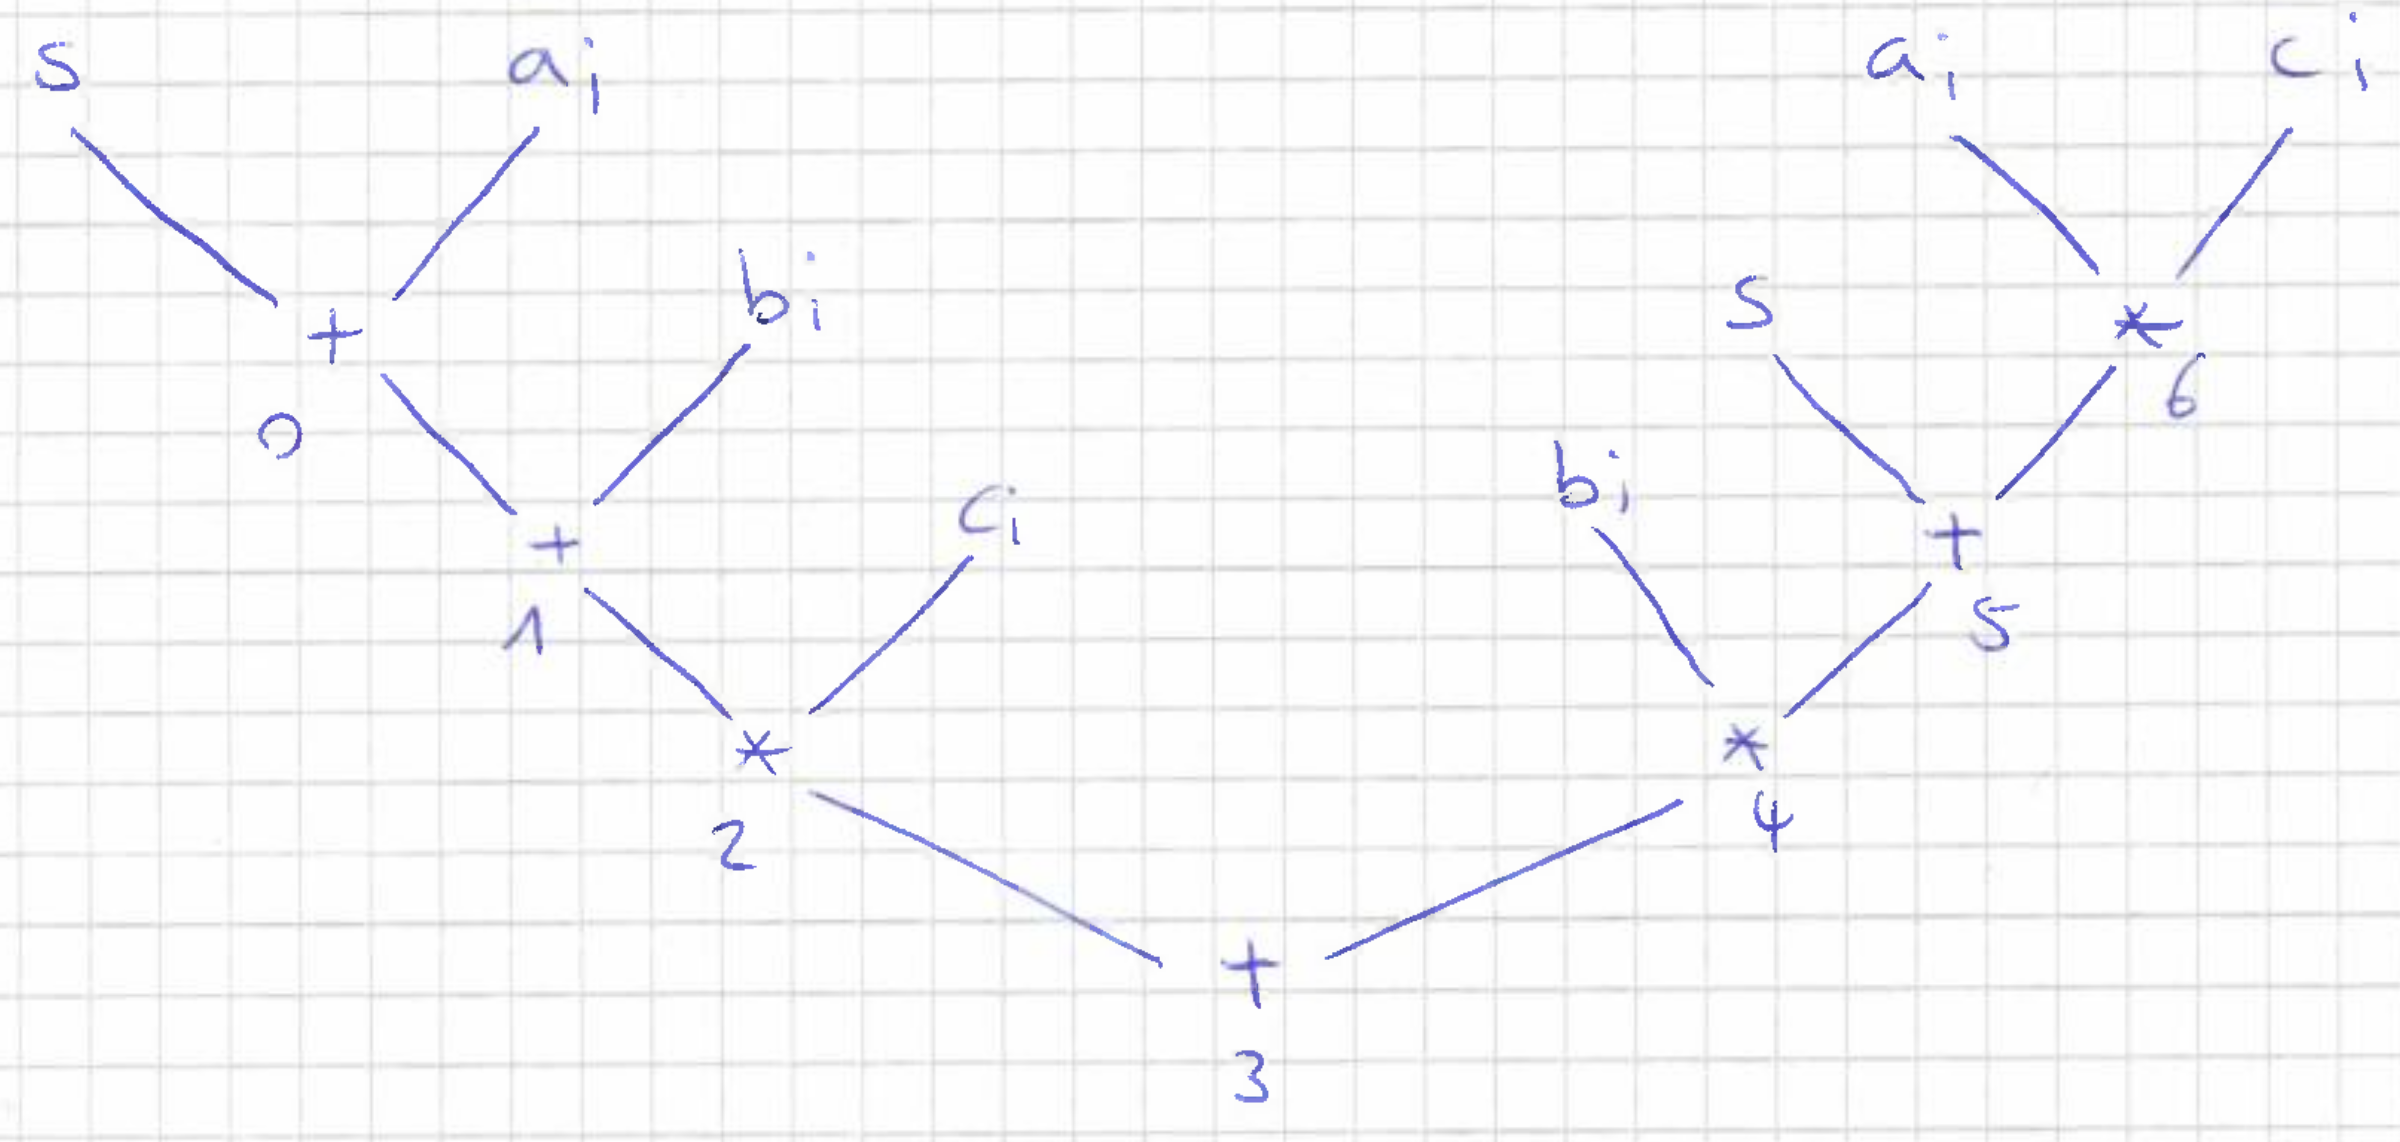
\includegraphics[width=0.8\textwidth]{normal_dep_tree.png}
        \end{center}
        Next, we have to distribute these operations on the available ports. The Haswell micro architecture can handle multiplications on port 0 and port 1 simultaneously. Additions can only be schedule on port 1. As we want a lower bound, we assume a perfect out-of-order execution which result in the following port assignment.
        
        \begin{center}
        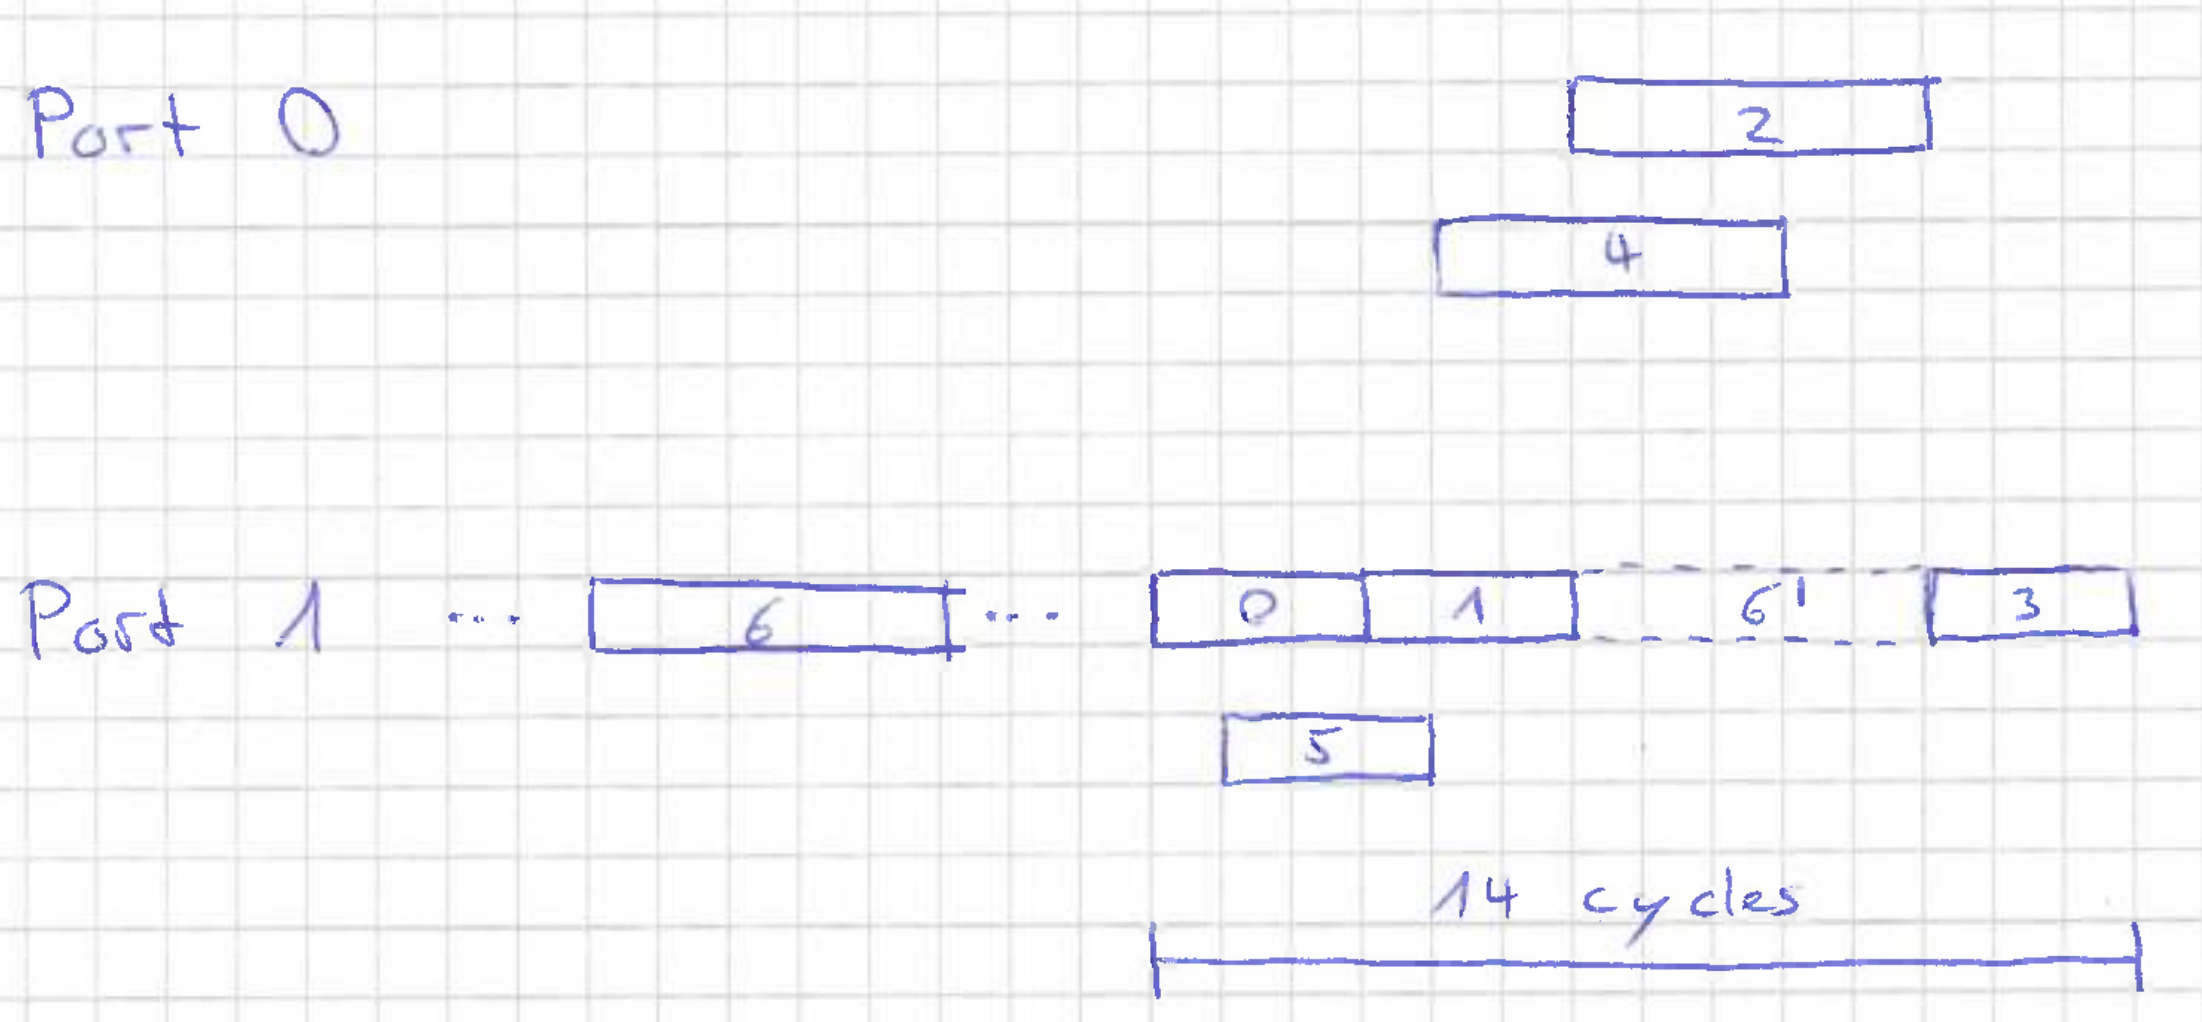
\includegraphics[width=0.8\textwidth]{normal_scheduling.png}
        \end{center}
        
        The operations are labeled according to the dependency tree. We can precompute operation 6 in the previous loop iteration (computation does not depend on results of the previous iteration). This allows us to execute operation 5 earlier. The precomputation of the next iteration is labeled as operation $6'$. Any other precomputation is not possible because all operations depends on results of the previous iteration.
        
        An optimal assignment with precomputation gives us a lower bound of $14 \cdot N$ cycles.
        
        \newpage
        
        \item In this part we consider FMA instructions and which is shown in the following dependency graph.
        \begin{center}
        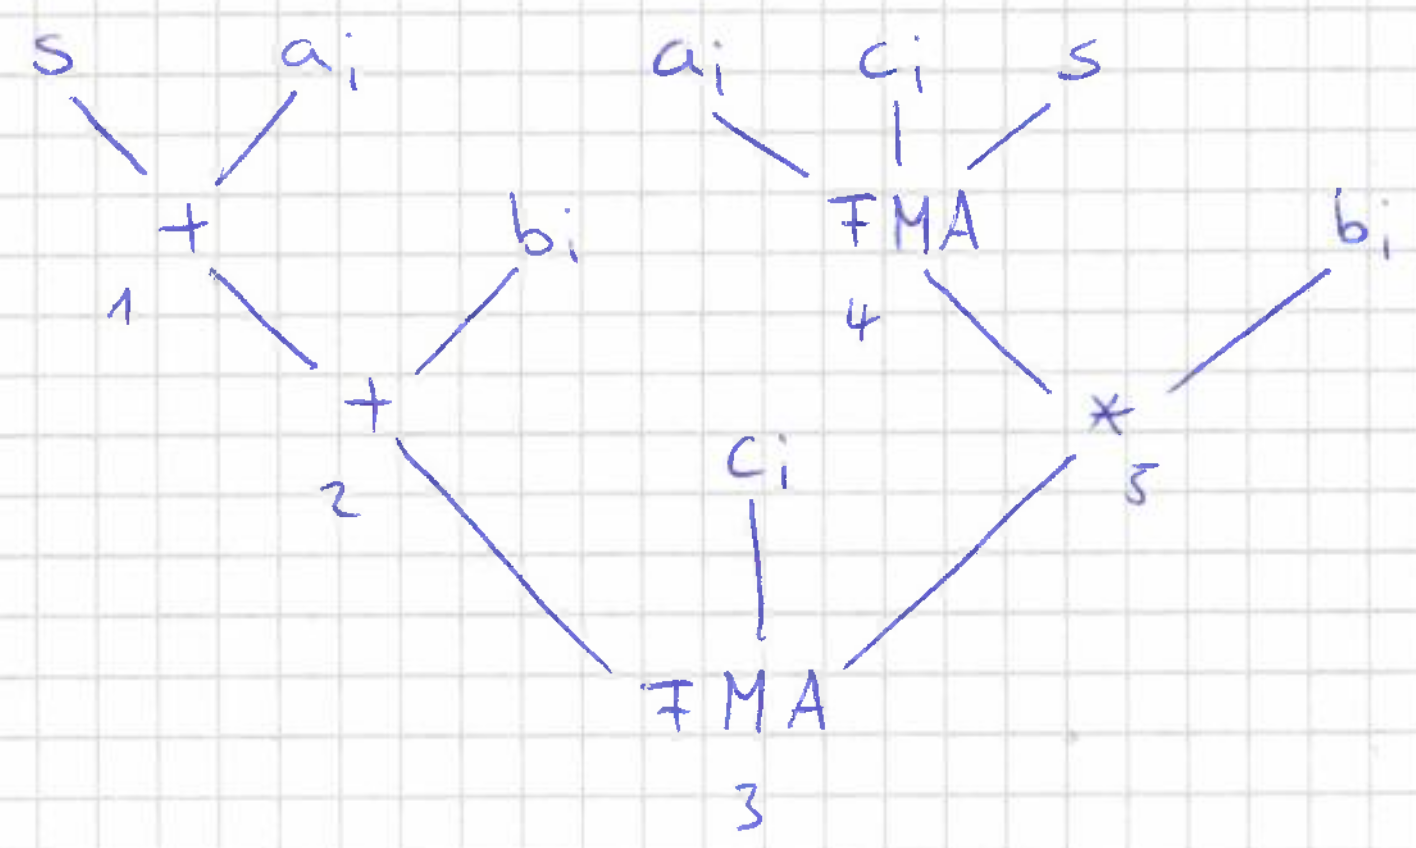
\includegraphics[width=0.8\textwidth]{fma_dep_tree.png}
        \end{center}
        We use FMAs as much as possible, which does not necessarily lead to the fastest execution. Haswell has a FMA unit on port 0 and port 1. Using this information we can construct the following port assignment.
        \begin{center}
        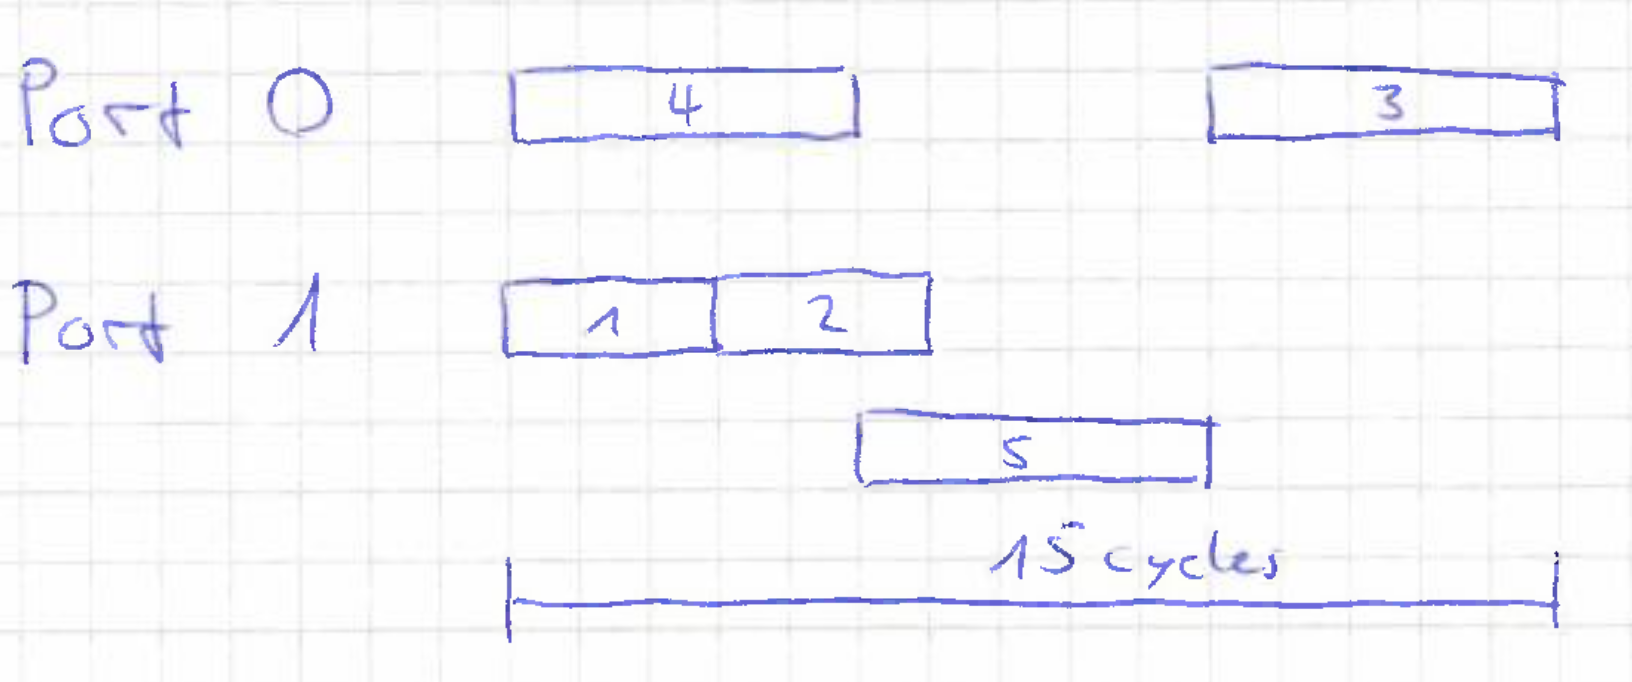
\includegraphics[width=0.8\textwidth]{fma_scheduling.png}
        \end{center}
        All operations are depended on the previous loop iteration or a intermediate result so we can consider this assignment as optimal. Using this assignment we get a lower bound of $15 \cdot N$.
    \end{enumerate}
\end{enumerate}

\printbibliography

\end{document}
